% GNUPLOT: LaTeX picture with Postscript
\begingroup
  \makeatletter
  \providecommand\color[2][]{%
    \GenericError{(gnuplot) \space\space\space\@spaces}{%
      Package color not loaded in conjunction with
      terminal option `colourtext'%
    }{See the gnuplot documentation for explanation.%
    }{Either use 'blacktext' in gnuplot or load the package
      color.sty in LaTeX.}%
    \renewcommand\color[2][]{}%
  }%
  \providecommand\includegraphics[2][]{%
    \GenericError{(gnuplot) \space\space\space\@spaces}{%
      Package graphicx or graphics not loaded%
    }{See the gnuplot documentation for explanation.%
    }{The gnuplot epslatex terminal needs graphicx.sty or graphics.sty.}%
    \renewcommand\includegraphics[2][]{}%
  }%
  \providecommand\rotatebox[2]{#2}%
  \@ifundefined{ifGPcolor}{%
    \newif\ifGPcolor
    \GPcolortrue
  }{}%
  \@ifundefined{ifGPblacktext}{%
    \newif\ifGPblacktext
    \GPblacktexttrue
  }{}%
  % define a \g@addto@macro without @ in the name:
  \let\gplgaddtomacro\g@addto@macro
  % define empty templates for all commands taking text:
  \gdef\gplbacktext{}%
  \gdef\gplfronttext{}%
  \makeatother
  \ifGPblacktext
    % no textcolor at all
    \def\colorrgb#1{}%
    \def\colorgray#1{}%
  \else
    % gray or color?
    \ifGPcolor
      \def\colorrgb#1{\color[rgb]{#1}}%
      \def\colorgray#1{\color[gray]{#1}}%
      \expandafter\def\csname LTw\endcsname{\color{white}}%
      \expandafter\def\csname LTb\endcsname{\color{black}}%
      \expandafter\def\csname LTa\endcsname{\color{black}}%
      \expandafter\def\csname LT0\endcsname{\color[rgb]{1,0,0}}%
      \expandafter\def\csname LT1\endcsname{\color[rgb]{0,1,0}}%
      \expandafter\def\csname LT2\endcsname{\color[rgb]{0,0,1}}%
      \expandafter\def\csname LT3\endcsname{\color[rgb]{1,0,1}}%
      \expandafter\def\csname LT4\endcsname{\color[rgb]{0,1,1}}%
      \expandafter\def\csname LT5\endcsname{\color[rgb]{1,1,0}}%
      \expandafter\def\csname LT6\endcsname{\color[rgb]{0,0,0}}%
      \expandafter\def\csname LT7\endcsname{\color[rgb]{1,0.3,0}}%
      \expandafter\def\csname LT8\endcsname{\color[rgb]{0.5,0.5,0.5}}%
    \else
      % gray
      \def\colorrgb#1{\color{black}}%
      \def\colorgray#1{\color[gray]{#1}}%
      \expandafter\def\csname LTw\endcsname{\color{white}}%
      \expandafter\def\csname LTb\endcsname{\color{black}}%
      \expandafter\def\csname LTa\endcsname{\color{black}}%
      \expandafter\def\csname LT0\endcsname{\color{black}}%
      \expandafter\def\csname LT1\endcsname{\color{black}}%
      \expandafter\def\csname LT2\endcsname{\color{black}}%
      \expandafter\def\csname LT3\endcsname{\color{black}}%
      \expandafter\def\csname LT4\endcsname{\color{black}}%
      \expandafter\def\csname LT5\endcsname{\color{black}}%
      \expandafter\def\csname LT6\endcsname{\color{black}}%
      \expandafter\def\csname LT7\endcsname{\color{black}}%
      \expandafter\def\csname LT8\endcsname{\color{black}}%
    \fi
  \fi
  \setlength{\unitlength}{0.0500bp}%
  \begin{picture}(7200.00,3600.00)%
    \gplgaddtomacro\gplbacktext{%
      \csname LTb\endcsname%
      \put(951,595){\makebox(0,0)[r]{\strut{} 0}}%
      \csname LTb\endcsname%
      \put(951,875){\makebox(0,0)[r]{\strut{} 5000}}%
      \csname LTb\endcsname%
      \put(951,1155){\makebox(0,0)[r]{\strut{} 10000}}%
      \csname LTb\endcsname%
      \put(951,1435){\makebox(0,0)[r]{\strut{} 15000}}%
      \csname LTb\endcsname%
      \put(951,1715){\makebox(0,0)[r]{\strut{} 20000}}%
      \csname LTb\endcsname%
      \put(951,1995){\makebox(0,0)[r]{\strut{} 25000}}%
      \csname LTb\endcsname%
      \put(951,2275){\makebox(0,0)[r]{\strut{} 30000}}%
      \csname LTb\endcsname%
      \put(951,2555){\makebox(0,0)[r]{\strut{} 35000}}%
      \csname LTb\endcsname%
      \put(951,2835){\makebox(0,0)[r]{\strut{} 40000}}%
      \csname LTb\endcsname%
      \put(951,3115){\makebox(0,0)[r]{\strut{} 45000}}%
      \csname LTb\endcsname%
      \put(951,3395){\makebox(0,0)[r]{\strut{} 50000}}%
      \csname LTb\endcsname%
      \put(1053,409){\makebox(0,0){\strut{} 0}}%
      \csname LTb\endcsname%
      \put(1783,409){\makebox(0,0){\strut{} 256}}%
      \csname LTb\endcsname%
      \put(2513,409){\makebox(0,0){\strut{} 512}}%
      \csname LTb\endcsname%
      \put(3243,409){\makebox(0,0){\strut{} 768}}%
      \csname LTb\endcsname%
      \put(3973,409){\makebox(0,0){\strut{} 1024}}%
      \csname LTb\endcsname%
      \put(4703,409){\makebox(0,0){\strut{} 1280}}%
      \csname LTb\endcsname%
      \put(5433,409){\makebox(0,0){\strut{} 1536}}%
      \csname LTb\endcsname%
      \put(6163,409){\makebox(0,0){\strut{} 1792}}%
      \csname LTb\endcsname%
      \put(6893,409){\makebox(0,0){\strut{} 2048}}%
      \csname LTb\endcsname%
      \put(144,1995){\rotatebox{-270}{\makebox(0,0){\strut{}Compute Time ($ms$)}}}%
      \csname LTb\endcsname%
      \put(3973,130){\makebox(0,0){\strut{}Number of Bodies ($n$)}}%
    }%
    \gplgaddtomacro\gplfronttext{%
      \csname LTb\endcsname%
      \put(2277,3228){\makebox(0,0)[r]{\strut{}Serial}}%
      \csname LTb\endcsname%
      \put(2277,3042){\makebox(0,0)[r]{\strut{}All OpenMP}}%
      \csname LTb\endcsname%
      \put(2277,2856){\makebox(0,0)[r]{\strut{}$1$ Level GPU}}%
      \csname LTb\endcsname%
      \put(2277,2670){\makebox(0,0)[r]{\strut{}$3$ Level GPU}}%
      \csname LTb\endcsname%
      \put(2277,2484){\makebox(0,0)[r]{\strut{}$6$ Level GPU}}%
      \csname LTb\endcsname%
      \put(2277,2298){\makebox(0,0)[r]{\strut{}All GPU}}%
    }%
    \gplbacktext
    \put(0,0){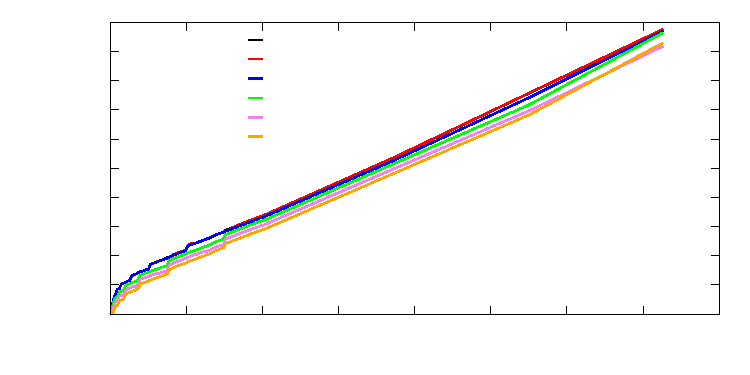
\includegraphics{speed}}%
    \gplfronttext
  \end{picture}%
\endgroup
